\section{Basics}

\subsection{Evolutionary Algorithms} \label{sec:EA}

Evolutionary algorithms are population-based metaheuristics \cite{EA}. Metaheuristics are methods for solving optimization problems by iteratively improving candidate solutions in relation to a given quality measure.
Population-based metaheuristics use populations of multiple solutions and iteratively change populations to find a good solution.
An evolutionary algorithm is based on a population $P$ of possible solutions $e_i \in P$ for the optimization problem or heuristic to be solved. A solution is also referred to as an individual in the context of population-based metaheuristics.

In general, evolutionary algorithms consist of the following steps \cite{EA}:

\begin{enumerate}
\item Initialization: The initial population of individuals is generated randomly.

\item Evolutionary process: The individuals are evaluated by calculating their fitness. Therefore a fitness function is needed.
According to their fitness, some of the individuals are selected to be the parents of the following generation.
Then a process with reproduction, recombination, and mutation starts - similar to biological processes.
The parents are being recombinated and the resulting individuals are mutated to form the offspring of the current generation.
These steps are being repeated until a new population of individuals is generated. The parents are also added to the new population. This new population substitutes the old population and the process is repeated until an abort criterion is fulfilled  (see figure \ref{fig:EA}).

\item The best individual is selected.
\end{enumerate}


\begin{figure}
	\begin{center}
		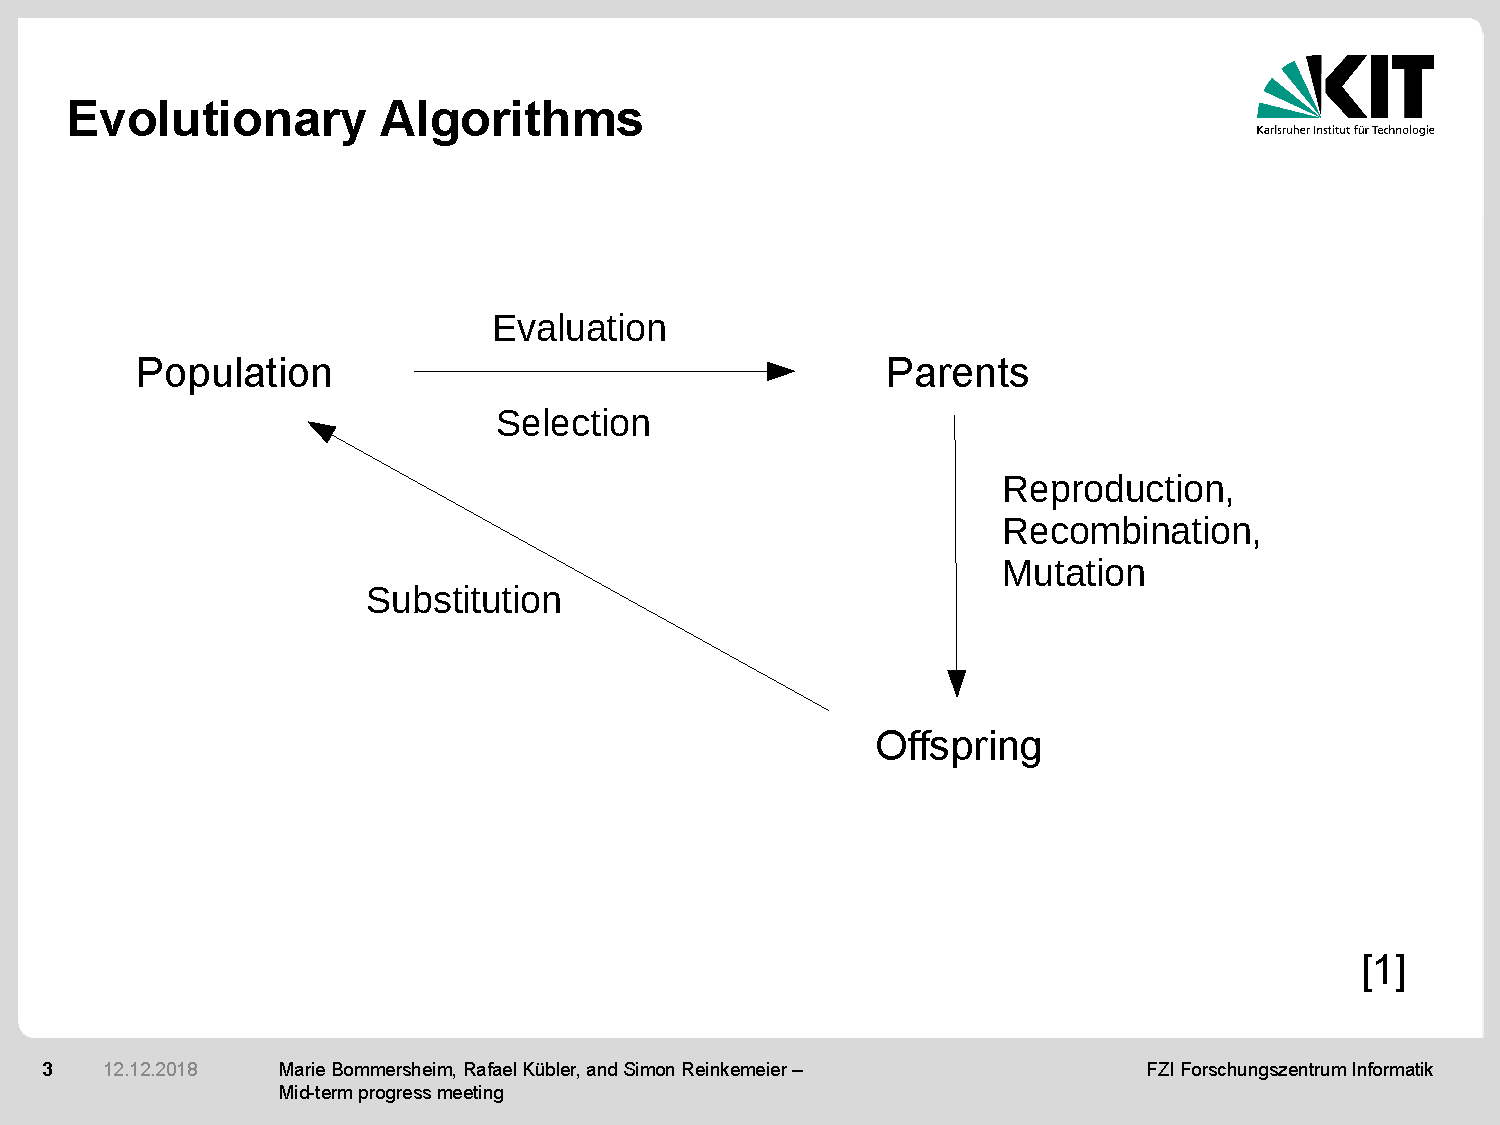
\includegraphics[trim = 2.2cm 6cm 4.1cm 6cm, clip, width=0.4\textwidth]{EA}
	\end{center}
	\caption{Evolutionary algorithms, adapted from \cite{EA}}
	\label{fig:EA}
\end{figure}

This approach brings with it a further question to ask. The exploitation vs exploration problem here can also be found in the number of generations vs the number of offspring per generation. A large number of offspring means a larger explorative phase, a higher number of generations a higher amount of exploitation.

\subsection{Monte Carlo Markov Chain} \label{sec:MCMC}

Monte Carlo Markov Chain algorithms can be used for hard optimization problems. The idea is similar to that of a greedy hillclimbing algorithm, with the added possibility of not only making forward (or "upward") steps, but also probabilistically accepting downhill steps. This is useful for getting over smaller local minima (see figure \ref{fig:MCMC1}) \cite{MCMC}. The decision to accept or reject a proposal to go from Point 1 to Point 2 is based on the ratio of fitnesses of the two points: uphill steps are always accepted, small downhill steps are usually accepted but huge downhill steps are almost never accepted (see figure \ref{fig:MCMC2}). In our approach, the probability of accepting a move was (fitness of current movement)/(fitness of last movement). If the fitness of the current movement is greater, the current movement is always accepted, smaller "downhill" steps are often accepted and larger "downhill" steps are very rarely accepted. The idea of this approach is geared towards quickly making progress towards a "good" movement (a movement with a large fitness function) without needing many samples. This approach rests on the assumption that the fitness function is at least somewhat of a hill i.e. somewhat steadily climbing.


\begin{figure}
	\begin{center}
		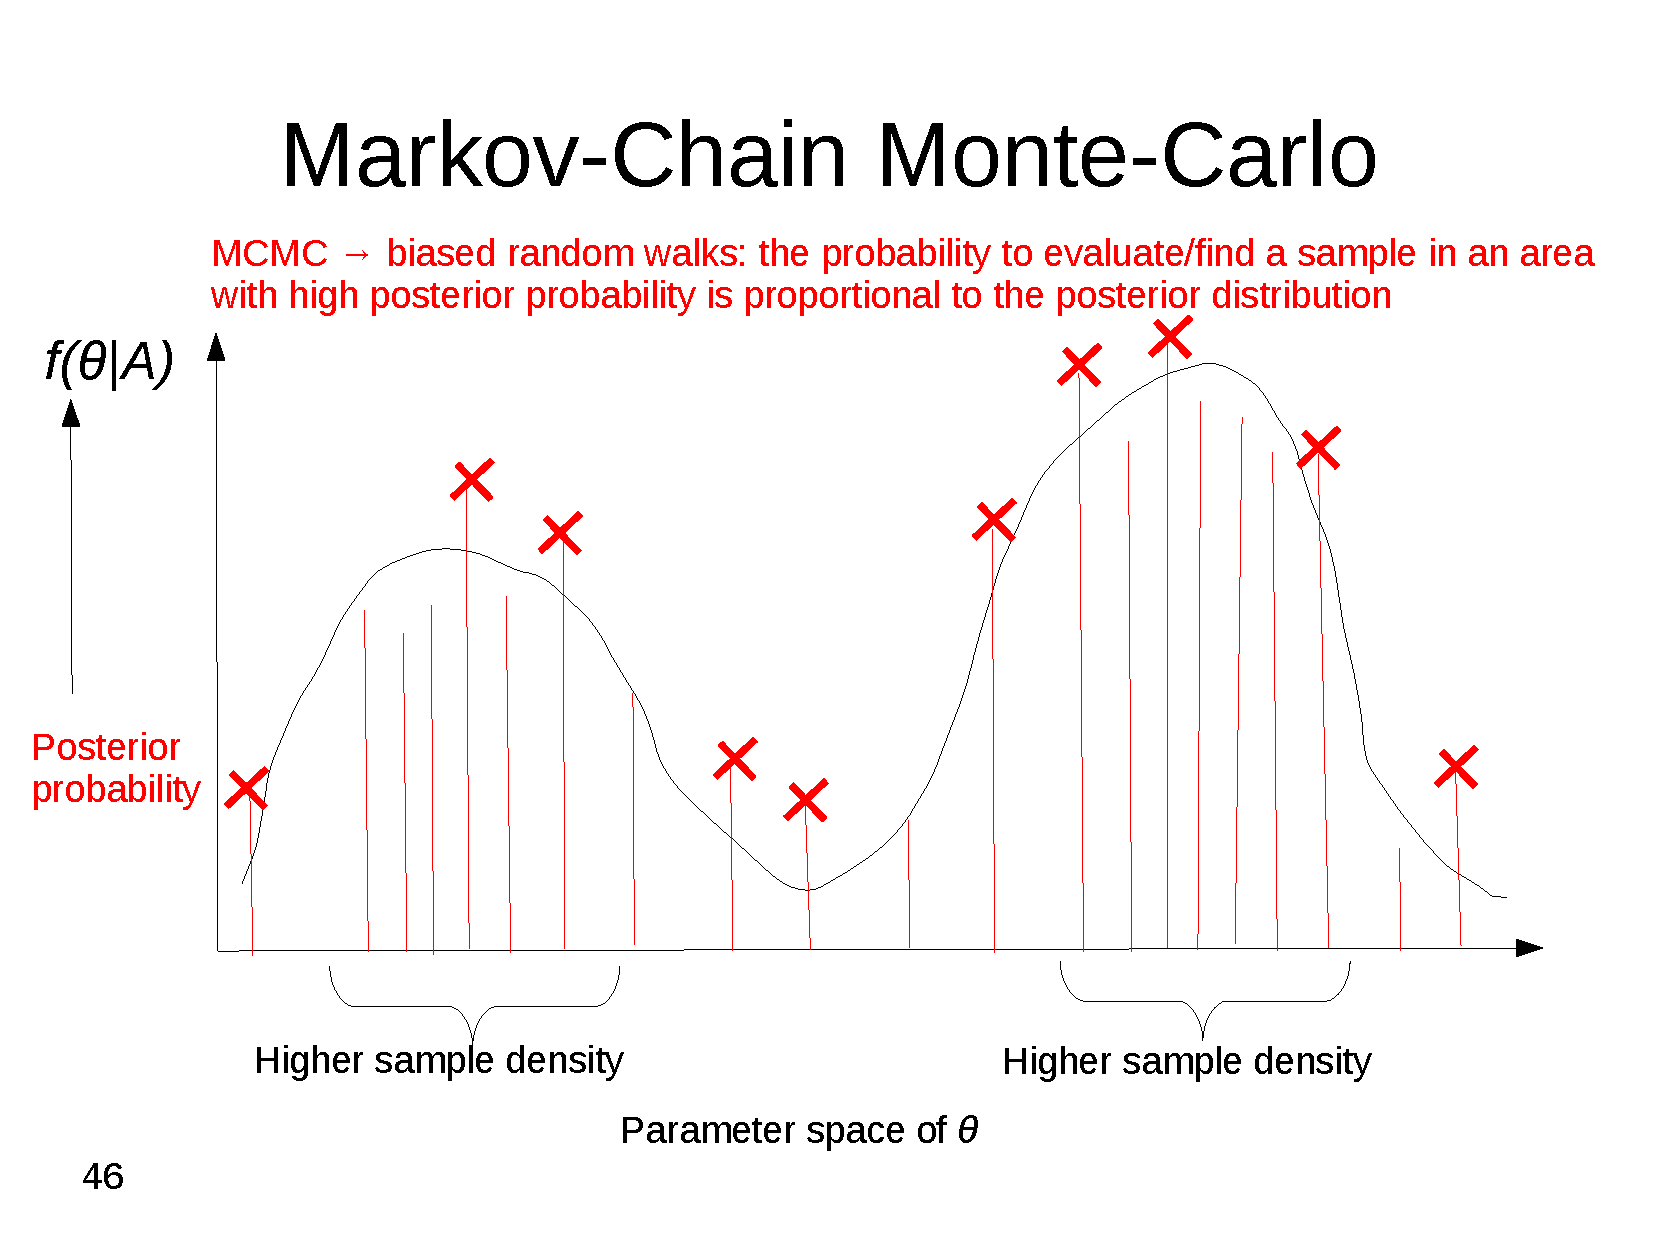
\includegraphics[trim = 0cm 1.5cm 1cm 5.4cm, clip, width=0.4\textwidth]{lecture12-seiten-46}
	\end{center}
	\caption{The probability to evaluate or find a sample in an area with high posterior probability is proportional to the posterior distribution, from \cite{MCMC}}
	\label{fig:MCMC1}
\end{figure}

\begin{figure}
	\begin{center}
		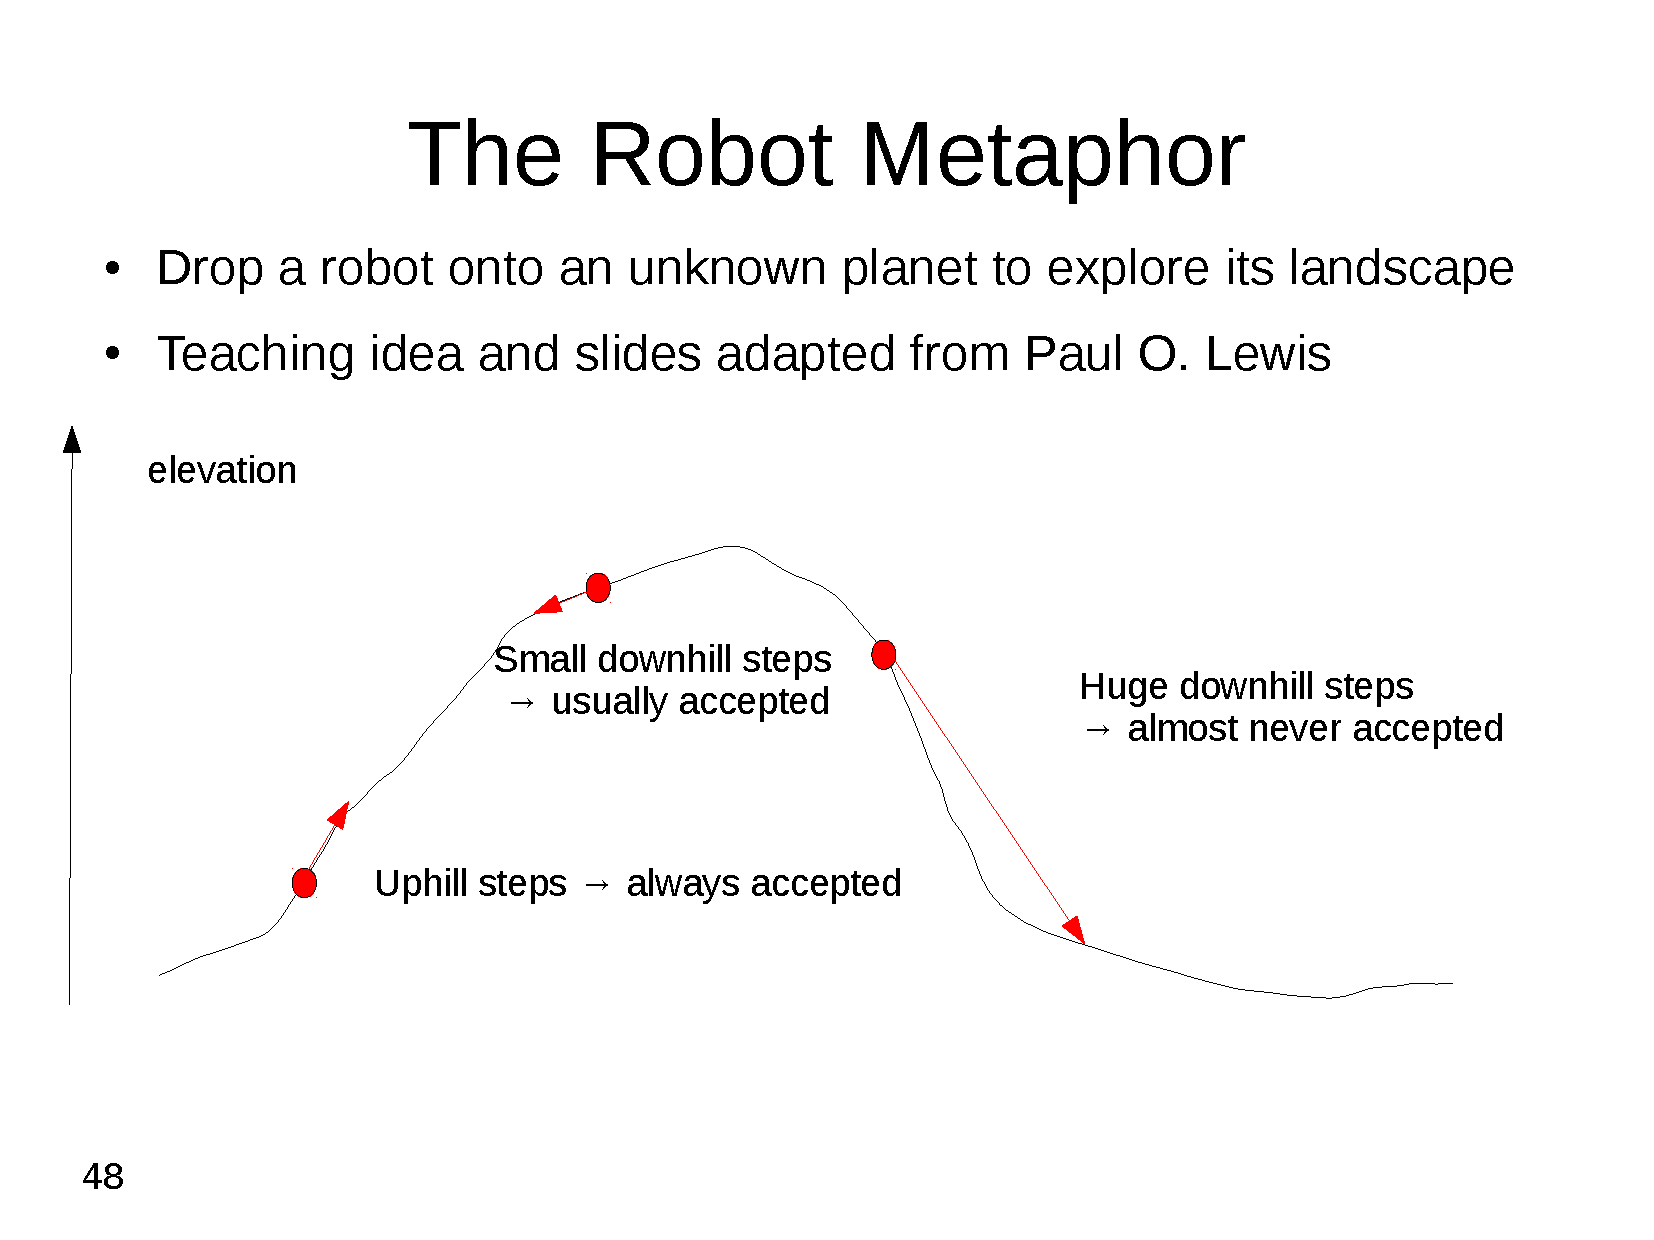
\includegraphics[trim = 0cm 4cm 1cm 7cm, clip, width=0.4\textwidth]{lecture12-seiten-48}
	\end{center}
	\caption{The decision to accept or reject a movement to go from Point 1 to Point 2 is based on the ratio of fitness functions of the two movements, from \cite{MCMC}}
	\label{fig:MCMC2}
\end{figure}